% !TEX root = main.tex
\chapter{Simulações e Resultados}
\label{cha:results}

A fim de melhorar as condições de reprodutibilidade das simulações realizadas neste trabalho, é importante observar a Tabela \ref{tab:results_pc_specs}, que traz as configurações do ambiente em que todas as simulações foram realizadas.

\begin{table}[H]
    \centering
    \caption{Ambiente de simulação.}
    \begin{tabular}{ll}
        \toprule
        \textbf{Componente} &   \textbf{Descrição}\\
        \midrule
        Processador         &   Intel Core i5-8600K 3.6 GHz (4.3 GHz Turbo) 6-Core 9 MB Cache\\
        CPU Cooler          &   Corsair H80i v2 Water Cooler\\
        Placa Mãe           &   Gigabyte Z370XP SLI\\
        Memória RAM         &   Corsair Vengeance DDR4 3000 MHz 16 GB (2 x 8 GB) C15\\
        SSD                 &   Kingston UV400 240 GB SATA III\\
        SSHD                &   Seagate Híbrido Firecuda 2 TB 64 MB Cache SATA III\\
        Placa de Vídeo      &   EVGA GTX 1080 Ti SC2 11 GB\\
        Fonte               &   Corsair CS750M\\
        Sistema Operacional &   Ubuntu Desktop 18.04 LTS 64-bit\\
        CUDA                &   v10.0\\
        CUDNN               &   v7.5\\
        PyTorch             &   v1.0.1\\
        \bottomrule
    \end{tabular}
    \label{tab:results_pc_specs}
\end{table}

A respeito do processador, apesar de a frequência de operação de 4.3 GHz ser atingida apenas por meio da função Turbo, essa função pode ficar ativada sempre que o processador detectar uma demanda por alto poder de processamento, o que pode ocorrer durante todo o período de processamento da simulação. A refrigeração da CPU foi feita por meio de uma solução relativamente poderosa, assim como a fonte utilizada possui capacidades consideravelmente superiores às demandadas, além de ser altamente estável e suficientemente eficiente; isso garantiu que nenhum dos resultados tenha sofrido interferências negativas por conta de qualquer questão inesperada e atípica relacionada ao \textit{Hardware}. Apesar de o computador possuir um SSHD, que é uma solução híbrida, o sistema operacional, os programas utilizados e todos os arquivos dos \textit{datasets} localizavam-se no SSD; o SSHD foi apenas utilizado para fins de \textit{Backup}.

Embora o PyTorch ofereça suporte a processamento por GPUs, várias etapas que envolvem processamento somente podem ser efetuadas por CPU, o que, inevitavelmente, faz com que haja um aumento no tempo demandado para concluir toda a simulação. Essa constatação pode ser efetuada por meio de monitores de recursos do sistema operacional e da placa de vídeo; no caso do Ubuntu, eles podem ser acessados por meio dos comandos \textbf{\$ htop} e \textbf{\$ nvidia-smi}, sendo que, caso se deseje visualizar o monitor de recursos da gpu com um intervalo de atualização de 1 segundo, pode-se utilizar o comando \textbf{\$ watch -n 1 nvidia-smi}.




\begin{figure}[H]
    \centering
    \subfigure[Época 0]
    {
        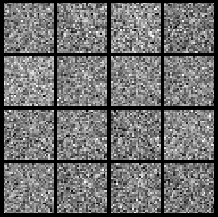
\includegraphics[width=0.30\textwidth]{figs/MNIST/new_tests/_epoch_0_batch_0.png}
        \label{fig:results_mnist_epoch-0}
    }
    \hspace{0.5cm}
    \subfigure[Época 3]
    {
        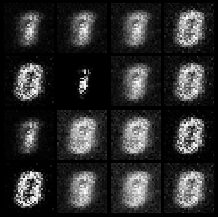
\includegraphics[width=0.30\textwidth]{figs/MNIST/new_tests/_epoch_3_batch_500.png}
        \label{fig:results_mnist_epoch-3}
    }
    \\
    \vspace{0.5cm}
    \subfigure[Época 32]
    {
        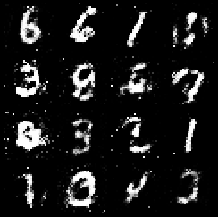
\includegraphics[width=0.30\textwidth]{figs/MNIST/new_tests/_epoch_32_batch_400.png}
        \label{fig:results_mnist_epoch-32}
    }
    \hspace{0.5cm}
    \subfigure[Época 299]
    {
        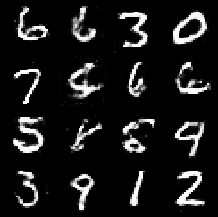
\includegraphics[width=0.30\textwidth]{figs/MNIST/new_tests/_epoch_299_batch_500.png}
        \label{fig:results_mnist_epoch-299}
    }
    \caption{Gerações da GAN \textit{Vanilla} para o \textit{dataset} MNIST em diferentes épocas.}
    \label{fig:results_mnist}
\end{figure}



\pagebreak
\newpage



\begin{figure}[H]
    \centering
    \subfigure[Erros]
    {
        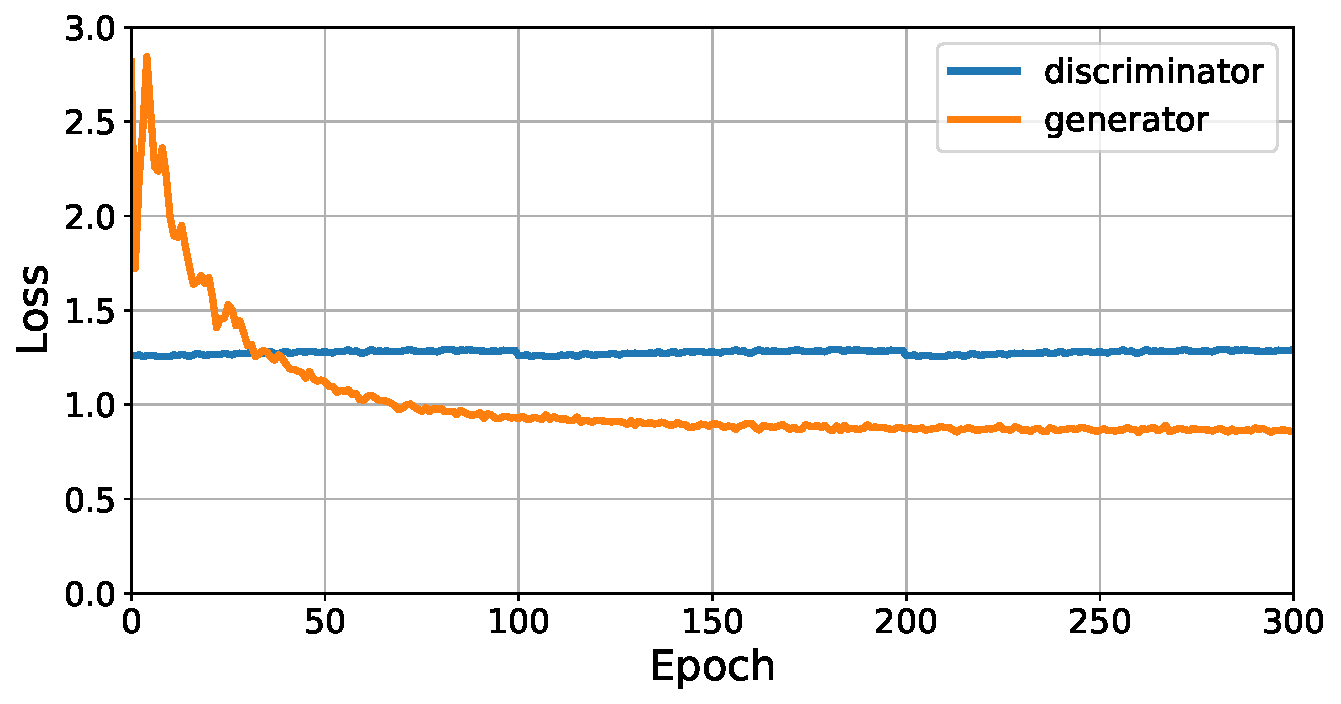
\includegraphics[width=0.75\textwidth]{figs/results/pytorch_vanilla_mnist_loss_0-299.pdf}
        \label{fig:results_pytorch_vanilla_mnist_loss}
    }
    \\
    \vspace{0.5cm}
    \subfigure[Incertezas]
    {
        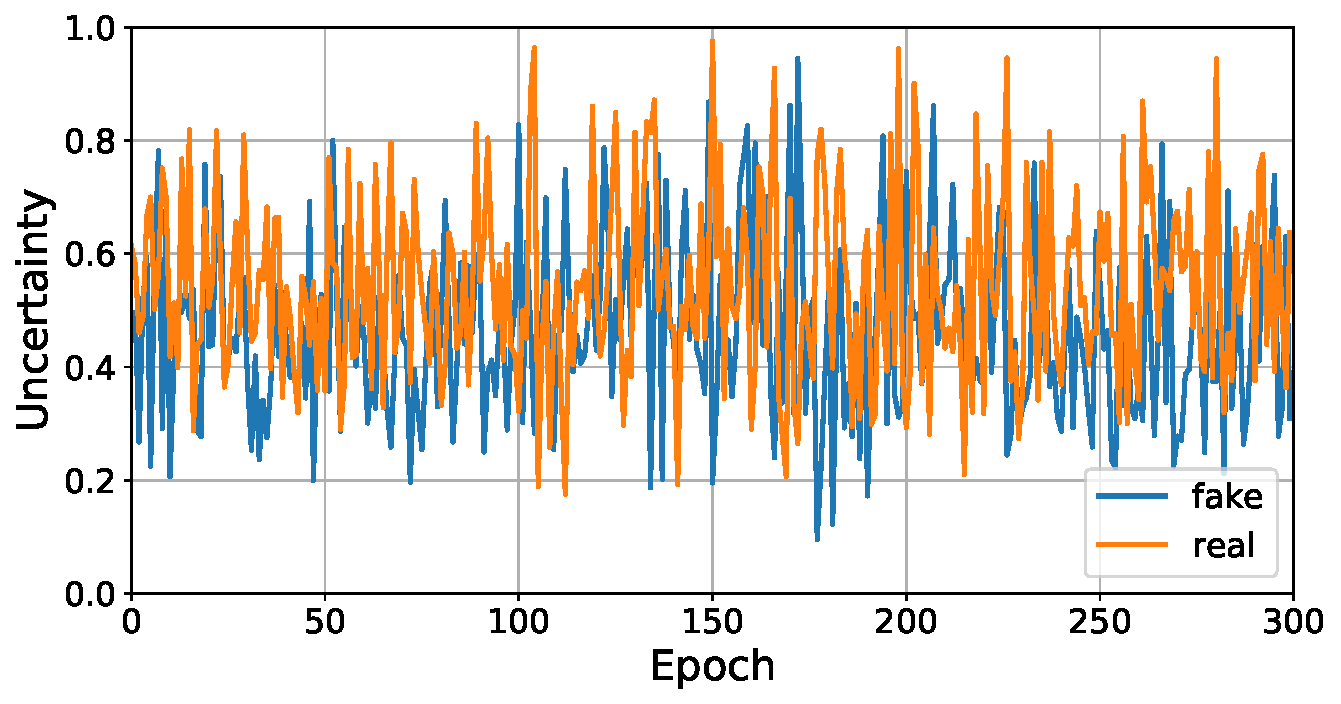
\includegraphics[width=0.75\textwidth]{figs/results/pytorch_vanilla_mnist_uncertainty_0-299.pdf}
        \label{fig:results_pytorch_vanilla_mnist_uncertainty}
    }
    \caption{Erros e incertezas da GAN \textit{Vanilla} para o \textit{dataset} MNIST em diferentes épocas.}
    \label{fig:results_pytorch_vanilla_mnist_scores}
\end{figure}